\documentclass[10pt,a4paper]{article}\usepackage[]{graphicx}\usepackage[]{color}
%% maxwidth is the original width if it is less than linewidth
%% otherwise use linewidth (to make sure the graphics do not exceed the margin)
\makeatletter
\def\maxwidth{ %
  \ifdim\Gin@nat@width>\linewidth
    \linewidth
  \else
    \Gin@nat@width
  \fi
}
\makeatother

\definecolor{fgcolor}{rgb}{0.345, 0.345, 0.345}
\newcommand{\hlnum}[1]{\textcolor[rgb]{0.686,0.059,0.569}{#1}}%
\newcommand{\hlstr}[1]{\textcolor[rgb]{0.192,0.494,0.8}{#1}}%
\newcommand{\hlcom}[1]{\textcolor[rgb]{0.678,0.584,0.686}{\textit{#1}}}%
\newcommand{\hlopt}[1]{\textcolor[rgb]{0,0,0}{#1}}%
\newcommand{\hlstd}[1]{\textcolor[rgb]{0.345,0.345,0.345}{#1}}%
\newcommand{\hlkwa}[1]{\textcolor[rgb]{0.161,0.373,0.58}{\textbf{#1}}}%
\newcommand{\hlkwb}[1]{\textcolor[rgb]{0.69,0.353,0.396}{#1}}%
\newcommand{\hlkwc}[1]{\textcolor[rgb]{0.333,0.667,0.333}{#1}}%
\newcommand{\hlkwd}[1]{\textcolor[rgb]{0.737,0.353,0.396}{\textbf{#1}}}%

\usepackage{framed}
\makeatletter
\newenvironment{kframe}{%
 \def\at@end@of@kframe{}%
 \ifinner\ifhmode%
  \def\at@end@of@kframe{\end{minipage}}%
  \begin{minipage}{\columnwidth}%
 \fi\fi%
 \def\FrameCommand##1{\hskip\@totalleftmargin \hskip-\fboxsep
 \colorbox{shadecolor}{##1}\hskip-\fboxsep
     % There is no \\@totalrightmargin, so:
     \hskip-\linewidth \hskip-\@totalleftmargin \hskip\columnwidth}%
 \MakeFramed {\advance\hsize-\width
   \@totalleftmargin\z@ \linewidth\hsize
   \@setminipage}}%
 {\par\unskip\endMakeFramed%
 \at@end@of@kframe}
\makeatother

\definecolor{shadecolor}{rgb}{.97, .97, .97}
\definecolor{messagecolor}{rgb}{0, 0, 0}
\definecolor{warningcolor}{rgb}{1, 0, 1}
\definecolor{errorcolor}{rgb}{1, 0, 0}
\newenvironment{knitrout}{}{} % an empty environment to be redefined in TeX

\usepackage{alltt}

\usepackage[T1]{fontenc}
\usepackage[polish]{babel}
\usepackage[cp1250]{inputenc}
\usepackage{amsmath}
\usepackage{amsfonts}
\usepackage{graphicx}
\usepackage{setspace}
\usepackage{savesym}
\savesymbol{arc}
\usepackage{color}
\usepackage{xcolor}
\usepackage{pict2e}
\usepackage{epstopdf}
\usepackage{geometry}

\newgeometry{tmargin=1.5cm, bmargin=1.5cm, lmargin=1.5cm, rmargin=1.5cm}
\pagestyle{empty}
\linespread{1.2}
\IfFileExists{upquote.sty}{\usepackage{upquote}}{}

\begin{document}

\section*{\centering PRACA DOMOWA 4\\ ASC - 31 maja 2014r.\\ \textbf{MARTA SOMMER} -- BSMAD -- 237503}

Analizujemy zbi�r \textit{Deaths}. Wczytajmy dane i zobaczmy, jak on wygl�da:

\begin{knitrout}
\definecolor{shadecolor}{rgb}{0.969, 0.969, 0.969}\color{fgcolor}\begin{kframe}
\begin{verbatim}
##        Jan   Feb   Mar   Apr   May   Jun   Jul   Aug   Sep   Oct   Nov
## 1973  9007  8106  8928  9137 10017 10826 11317 10744  9713  9938  9161
## 1974  7750  6981  8038  8422  8714  9512 10120  9823  8743  9129  8710
## 1975  8162  7306  8124  7870  9387  9556 10093  9620  8285  8433  8160
## 1976  7717  7461  7776  7925  8634  8945 10078  9179  8037  8488  7874
## 1977  7792  6957  7726  8106  8890  9299 10625  9302  8314  8850  8265
## 1978  7836  6892  7791  8129  9115  9434 10484  9827  9110  9070  8633
##        Dec
## 1973  8927
## 1974  8680
## 1975  8034
## 1976  8647
## 1977  8796
## 1978  9240
\end{verbatim}
\end{kframe}
\end{knitrout}


Wyestymujmy komponent� sezonow� i trend za pomoc� funkcji \texttt{decompose()}. Oto otrzymany wykres:

\begin{knitrout}
\definecolor{shadecolor}{rgb}{0.969, 0.969, 0.969}\color{fgcolor}

{\centering 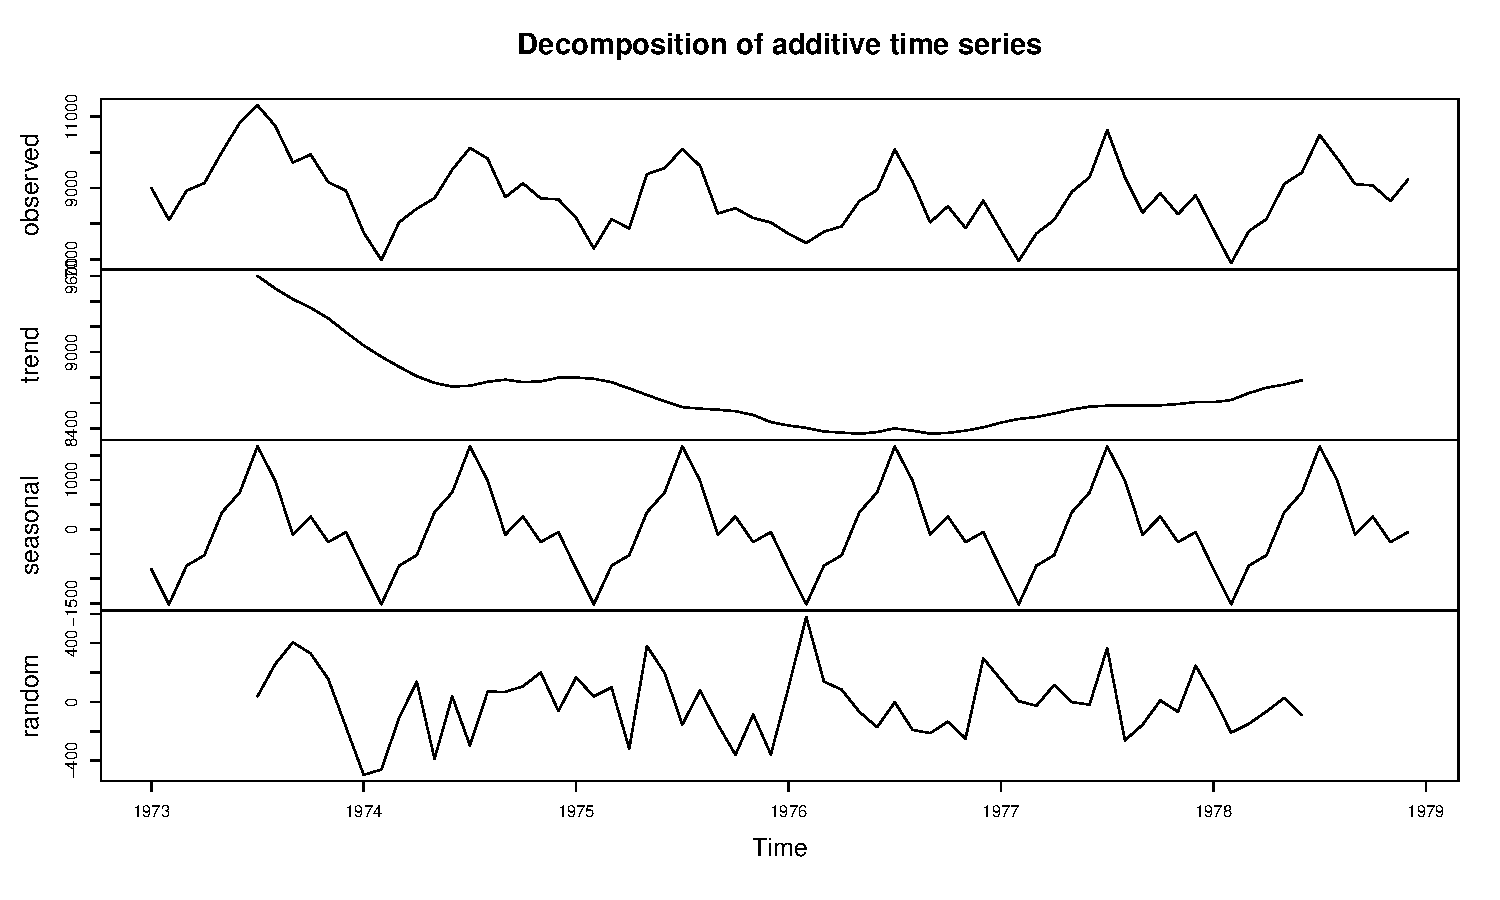
\includegraphics[width=\maxwidth]{figure/unnamed-chunk-2} 

}



\end{knitrout}


Zajmijmy si� teraz tylko komponent� sezonow�. Oto jej wykres:

\begin{knitrout}
\definecolor{shadecolor}{rgb}{0.969, 0.969, 0.969}\color{fgcolor}

{\centering 
\includegraphics[width=\maxwidth]{figure/unnamed-chunk-3} 

}



\end{knitrout}


Oto jej g�sto�� spektralna:

\begin{knitrout}
\definecolor{shadecolor}{rgb}{0.969, 0.969, 0.969}\color{fgcolor}

{\centering 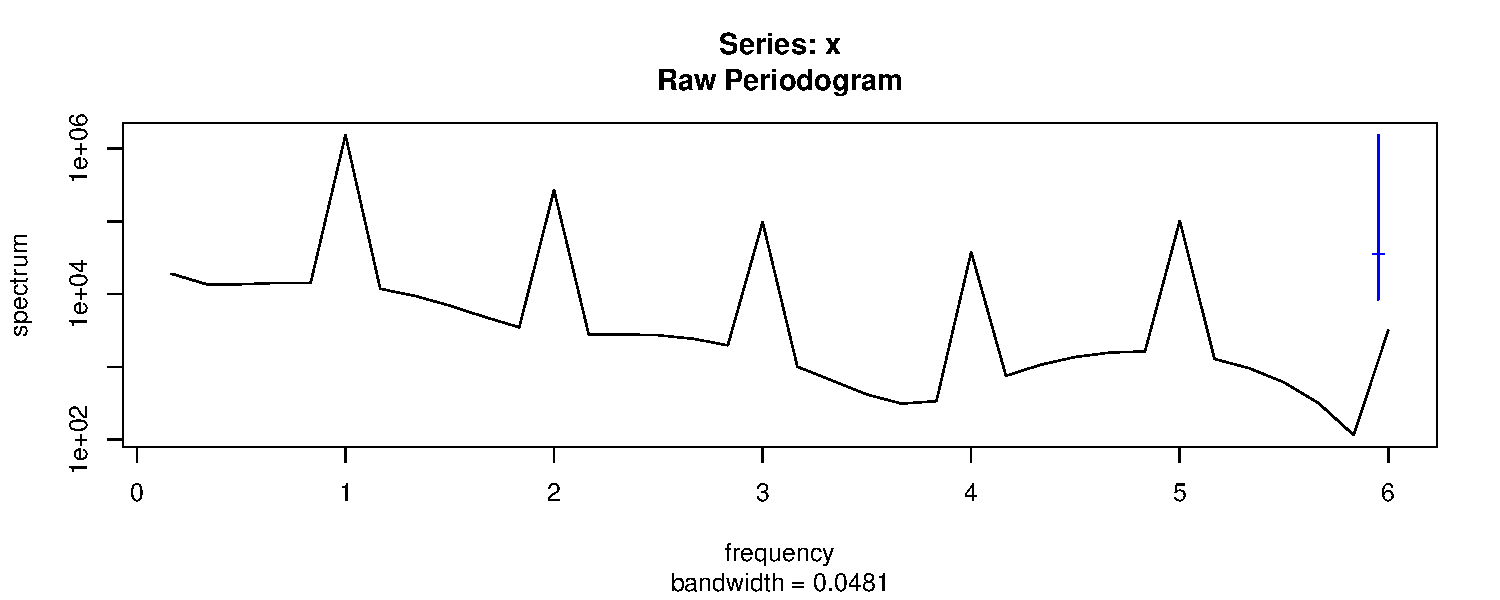
\includegraphics[width=\maxwidth]{figure/unnamed-chunk-4} 

}



\end{knitrout}


A oto jej dystrybuanta spektralna

\begin{knitrout}
\definecolor{shadecolor}{rgb}{0.969, 0.969, 0.969}\color{fgcolor}

{\centering 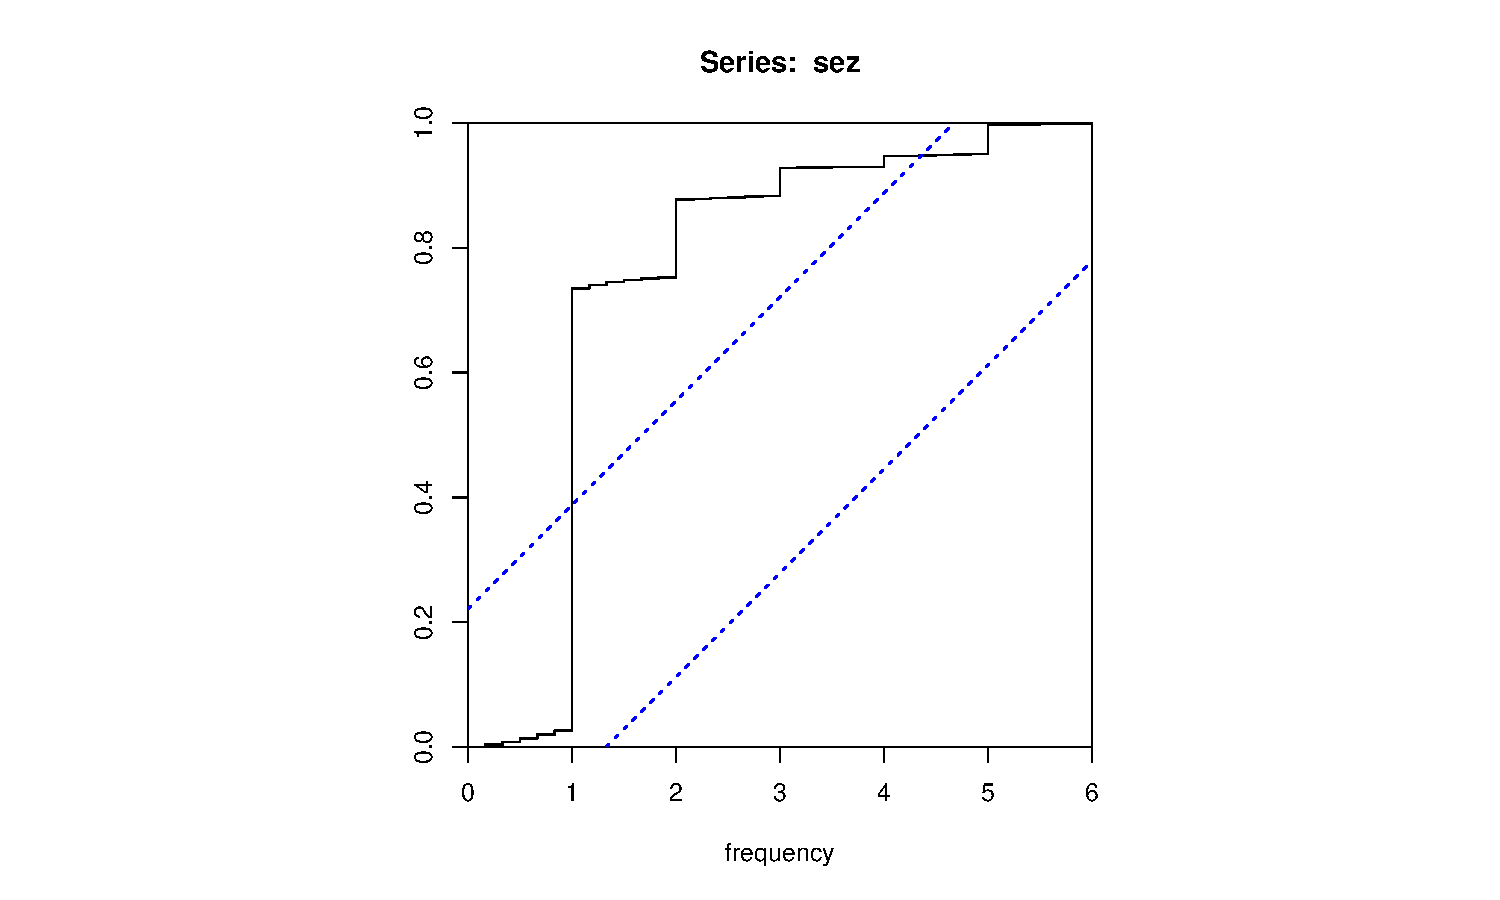
\includegraphics[width=\maxwidth]{figure/unnamed-chunk-5} 

}



\end{knitrout}


Na podstawie g�sto�ci spektralnej wyliczy�am, �e okres naszych danych wynosi $1$ rok, czyli $12$ miesi�cy.

\bigskip

Predykcja (wraz z przedzia�ami ufno�ci) dla kolejnych $36$ element�w:

\begin{knitrout}
\definecolor{shadecolor}{rgb}{0.969, 0.969, 0.969}\color{fgcolor}

{\centering 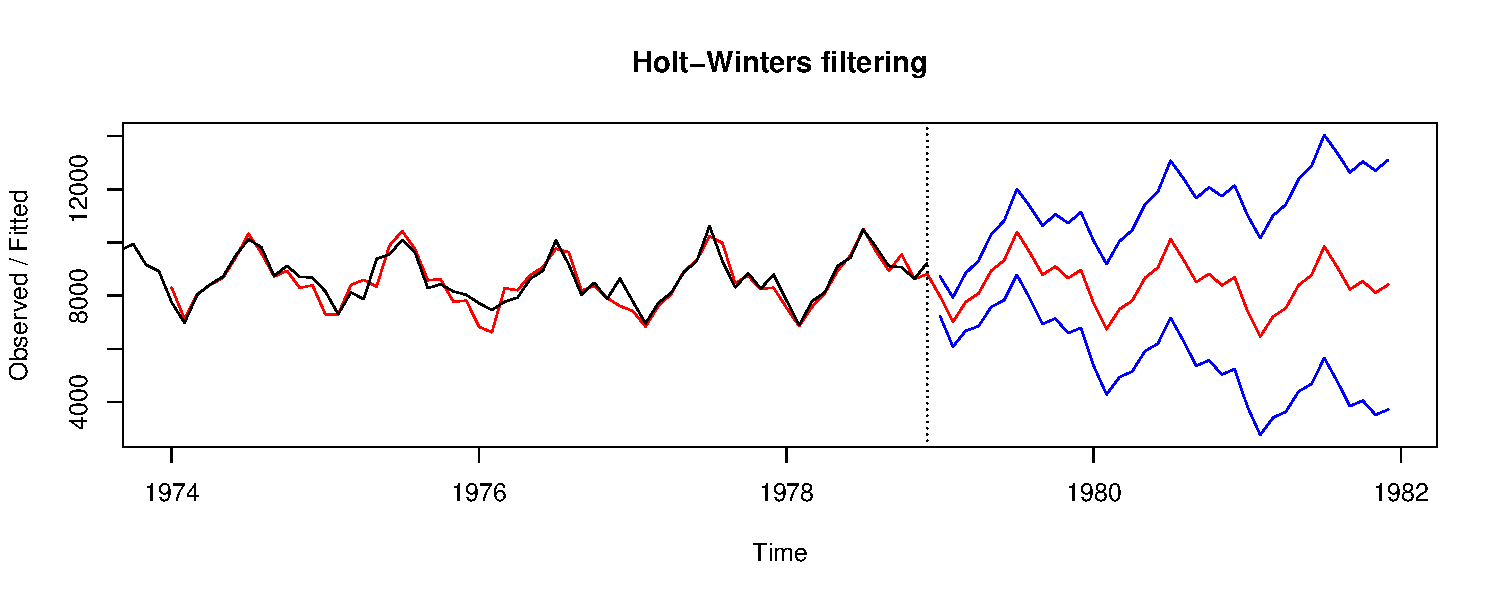
\includegraphics[width=\maxwidth]{figure/unnamed-chunk-6} 

}



\end{knitrout}


Dopasujmy model SARIMA korzystaj�c z kryterium AIC. Optymalny model wyszed� mi SARIMA$(1,1,1)(1,1,1)_{12}$. Przyjrzyjmy si� predykcji na tym modelu:




\begin{knitrout}
\definecolor{shadecolor}{rgb}{0.969, 0.969, 0.969}\color{fgcolor}

{\centering 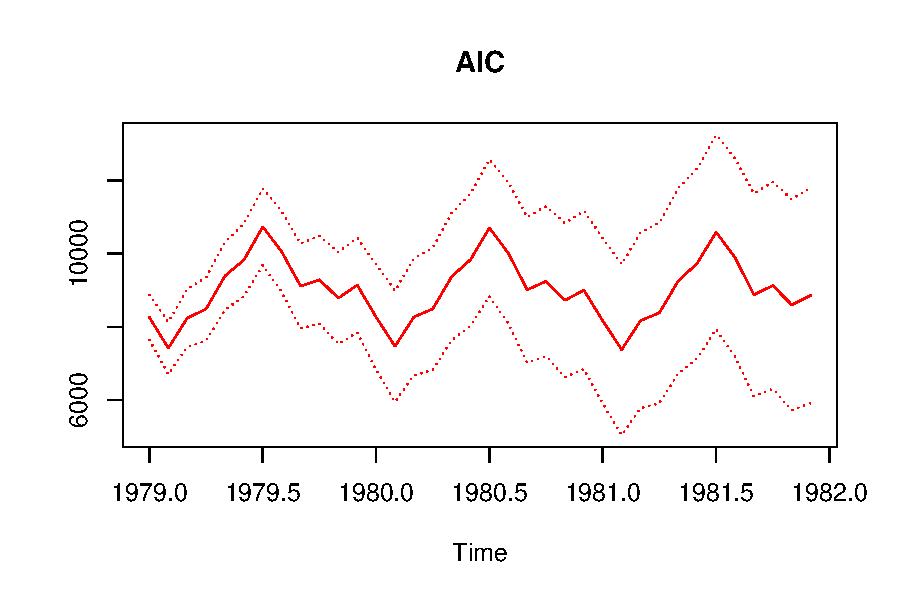
\includegraphics[width=\maxwidth]{figure/unnamed-chunk-8} 

}



\end{knitrout}


\section*{\textbf{\underline{Kod �r�d�owy}}}

\begin{knitrout}
\definecolor{shadecolor}{rgb}{0.969, 0.969, 0.969}\color{fgcolor}\begin{kframe}
\begin{alltt}
\hlcom{# praca domowa:}

\hlstd{d} \hlkwb{<-} \hlkwd{read.table}\hlstd{(}\hlstr{"C:\textbackslash{}\textbackslash{}Users\textbackslash{}\textbackslash{}Marta\textbackslash{}\textbackslash{}Desktop\textbackslash{}\textbackslash{}Marta\textbackslash{}\textbackslash{}studia\textbackslash{}\textbackslash{}rok4\textbackslash{}\textbackslash{}ASC\textbackslash{}\textbackslash{}DEATHS.DAT"}\hlstd{)}
\hlstd{d} \hlkwb{<-} \hlkwd{ts}\hlstd{(d,} \hlkwc{start} \hlstd{=} \hlnum{1973}\hlstd{,} \hlkwc{frequency} \hlstd{=} \hlnum{12}\hlstd{)}
\hlstd{d}

\hlcom{# a)}

\hlstd{dec} \hlkwb{<-} \hlkwd{decompose}\hlstd{(d)}
\hlkwd{plot}\hlstd{(dec)}

\hlstd{sez} \hlkwb{<-} \hlstd{dec}\hlopt{$}\hlstd{seasonal}
\hlkwd{plot}\hlstd{(sez)}
\hlstd{sp.sez} \hlkwb{<-} \hlkwd{spectrum}\hlstd{(sez)}
\hlkwd{cpgram}\hlstd{(sez)}
\hlstd{sp.sez}\hlopt{$}\hlstd{freq[}\hlkwd{order}\hlstd{(}\hlopt{-}\hlstd{sp.sez}\hlopt{$}\hlstd{spec)[}\hlnum{1}\hlstd{]]}  \hlcom{# okres co 1 rok}

\hlstd{m} \hlkwb{<-} \hlkwd{HoltWinters}\hlstd{(d,} \hlkwc{seasonal} \hlstd{=} \hlstr{"additive"}\hlstd{)}
\hlstd{p} \hlkwb{<-} \hlkwd{predict}\hlstd{(m,} \hlkwc{n.ahead} \hlstd{=} \hlnum{36}\hlstd{,} \hlkwc{prediction.interval} \hlstd{=} \hlnum{TRUE}\hlstd{)}
\hlkwd{plot}\hlstd{(m, p)}

\hlcom{# b)}

\hlstd{tab} \hlkwb{<-} \hlkwd{array}\hlstd{(}\hlnum{0}\hlstd{,} \hlkwc{dim} \hlstd{=} \hlkwd{c}\hlstd{(}\hlnum{2}\hlstd{,} \hlnum{2}\hlstd{,} \hlnum{2}\hlstd{,} \hlnum{2}\hlstd{),} \hlkwc{dimnames} \hlstd{=} \hlkwd{c}\hlstd{(}\hlstr{"p"}\hlstd{,} \hlstr{"q"}\hlstd{,} \hlstr{"P"}\hlstd{,} \hlstr{"Q"}\hlstd{))}

\hlkwa{for} \hlstd{(i} \hlkwa{in} \hlnum{0}\hlopt{:}\hlnum{1}\hlstd{) \{}
    \hlkwa{for} \hlstd{(j} \hlkwa{in} \hlnum{0}\hlopt{:}\hlnum{1}\hlstd{) \{}
        \hlkwa{for} \hlstd{(k} \hlkwa{in} \hlnum{0}\hlopt{:}\hlnum{1}\hlstd{) \{}
            \hlkwa{for} \hlstd{(l} \hlkwa{in} \hlnum{0}\hlopt{:}\hlnum{1}\hlstd{) \{}
                \hlstd{tab[i} \hlopt{+} \hlnum{1}\hlstd{, j} \hlopt{+} \hlnum{1}\hlstd{, k} \hlopt{+} \hlnum{1}\hlstd{, l} \hlopt{+} \hlnum{1}\hlstd{]} \hlkwb{<-} \hlkwd{AIC}\hlstd{(}\hlkwd{arima}\hlstd{(d,} \hlkwc{order} \hlstd{=} \hlkwd{c}\hlstd{(i,}
                  \hlnum{1}\hlstd{, j),} \hlkwc{seasonal} \hlstd{=} \hlkwd{list}\hlstd{(}\hlkwc{order} \hlstd{=} \hlkwd{c}\hlstd{(k,} \hlnum{1}\hlstd{, l),} \hlkwc{period} \hlstd{=} \hlnum{12}\hlstd{),} \hlkwc{optim.control} \hlstd{=} \hlkwd{list}\hlstd{(}\hlkwc{maxit} \hlstd{=} \hlnum{10}\hlopt{^}\hlnum{5}\hlstd{)))}
            \hlstd{\}}
        \hlstd{\}}
    \hlstd{\}}
\hlstd{\}}

\hlstd{tab}
\hlstd{tab} \hlopt{==} \hlkwd{max}\hlstd{(tab)}  \hlcom{# wybral 1,1,1,1}

\hlstd{aic} \hlkwb{<-} \hlkwd{arima}\hlstd{(d,} \hlkwc{order} \hlstd{=} \hlkwd{c}\hlstd{(}\hlnum{1}\hlstd{,} \hlnum{1}\hlstd{,} \hlnum{1}\hlstd{),} \hlkwc{seasonal} \hlstd{=} \hlkwd{list}\hlstd{(}\hlkwc{order} \hlstd{=} \hlkwd{c}\hlstd{(}\hlnum{1}\hlstd{,} \hlnum{1}\hlstd{,} \hlnum{1}\hlstd{),} \hlkwc{period} \hlstd{=} \hlnum{12}\hlstd{))}
\hlstd{p} \hlkwb{<-} \hlkwd{predict}\hlstd{(aic,} \hlkwc{n.ahead} \hlstd{=} \hlnum{36}\hlstd{)}\hlopt{$}\hlstd{pred}
\hlstd{s} \hlkwb{<-} \hlkwd{predict}\hlstd{(aic,} \hlkwc{n.ahead} \hlstd{=} \hlnum{36}\hlstd{)}\hlopt{$}\hlstd{se}

\hlkwd{ts.plot}\hlstd{(p, p} \hlopt{+} \hlnum{2} \hlopt{*} \hlstd{s, p} \hlopt{-} \hlnum{2} \hlopt{*} \hlstd{s,} \hlkwc{col} \hlstd{=} \hlkwd{c}\hlstd{(}\hlstr{"red"}\hlstd{,} \hlstr{"red"}\hlstd{,} \hlstr{"red"}\hlstd{),} \hlkwc{lty} \hlstd{=} \hlkwd{c}\hlstd{(}\hlnum{1}\hlstd{,} \hlnum{3}\hlstd{,}
    \hlnum{3}\hlstd{),} \hlkwc{main} \hlstd{=} \hlstr{"AIC"}\hlstd{)}
\end{alltt}
\end{kframe}
\end{knitrout}



\end{document}



